\subsection{Model Testing}
Now take cases infected with Ebola in the distribution of West
African countries as an example \cite{bib5}(data see appendix
6), by each set of data, the number of days as the horizontal
and the number of infections to the vertical axis, to make a
scatter plot, as shown in Figure~\ref{fig:5}(A).
\begin{figure}
\centering
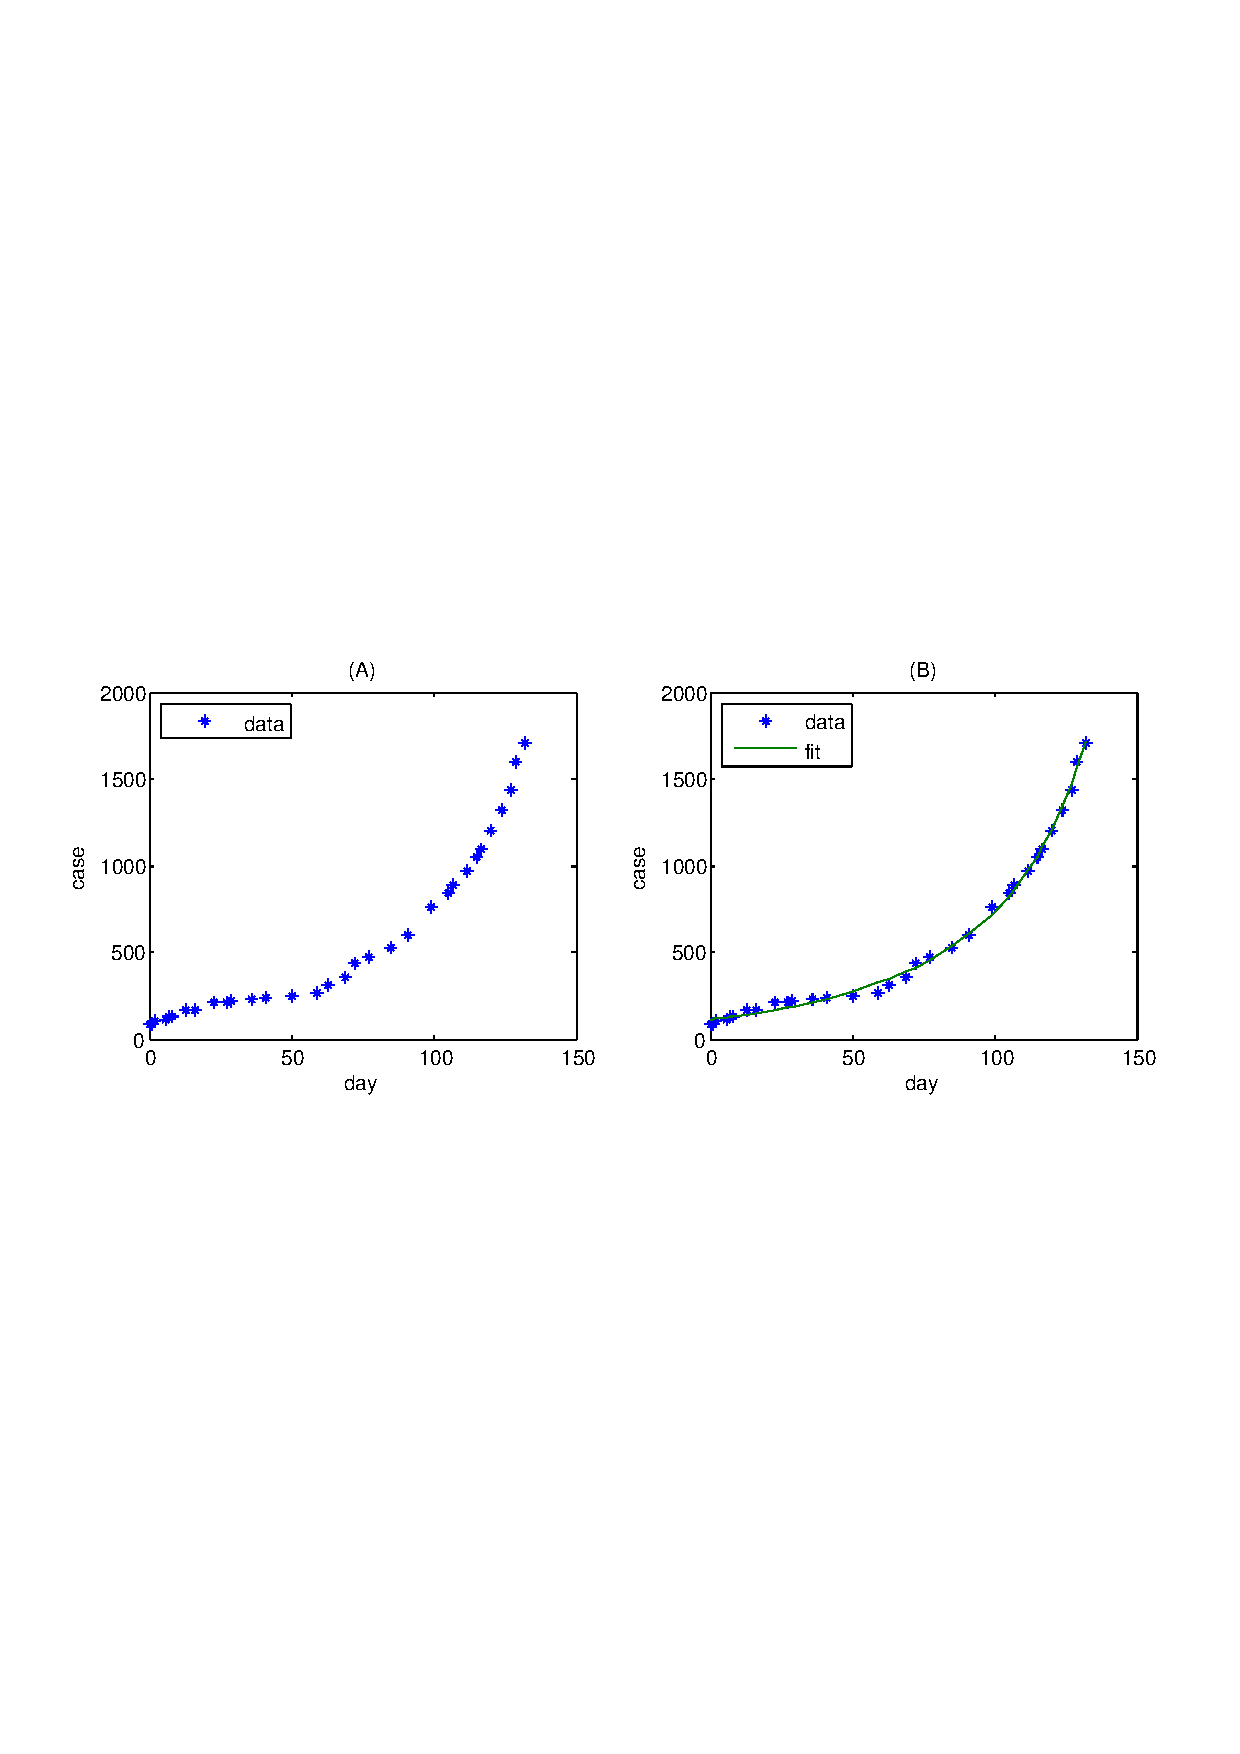
\includegraphics[width=4.7in]{imgs/sum_anly.pdf}
\caption{Statistic data and fitting}
\label{fig:5}
\end{figure}
Using MATLAB Statistics Toolbox function nlinfit, fitting
formula according to data:
\begin{equation}
i(t)=113e^{0.01748t}+0.2253e^{0.05946t}
\label{equ:14}
\end{equation}
The formula in line with graphs for Ebola
virus infection early on the case 2 in Section~\ref{sec:m1},
from Figure~\ref{fig:5}(B) we can see the data fit with good
results. It show that these assumptions and models
introduced is appropriate.
\subsection{Model Analysis}
Analyze data on the distribution of infection cases by Ebola 
in the West African countries and make fitting bias figure, as
shown in Figure~\ref{fig:6}.\\
\begin{figure}
\centering
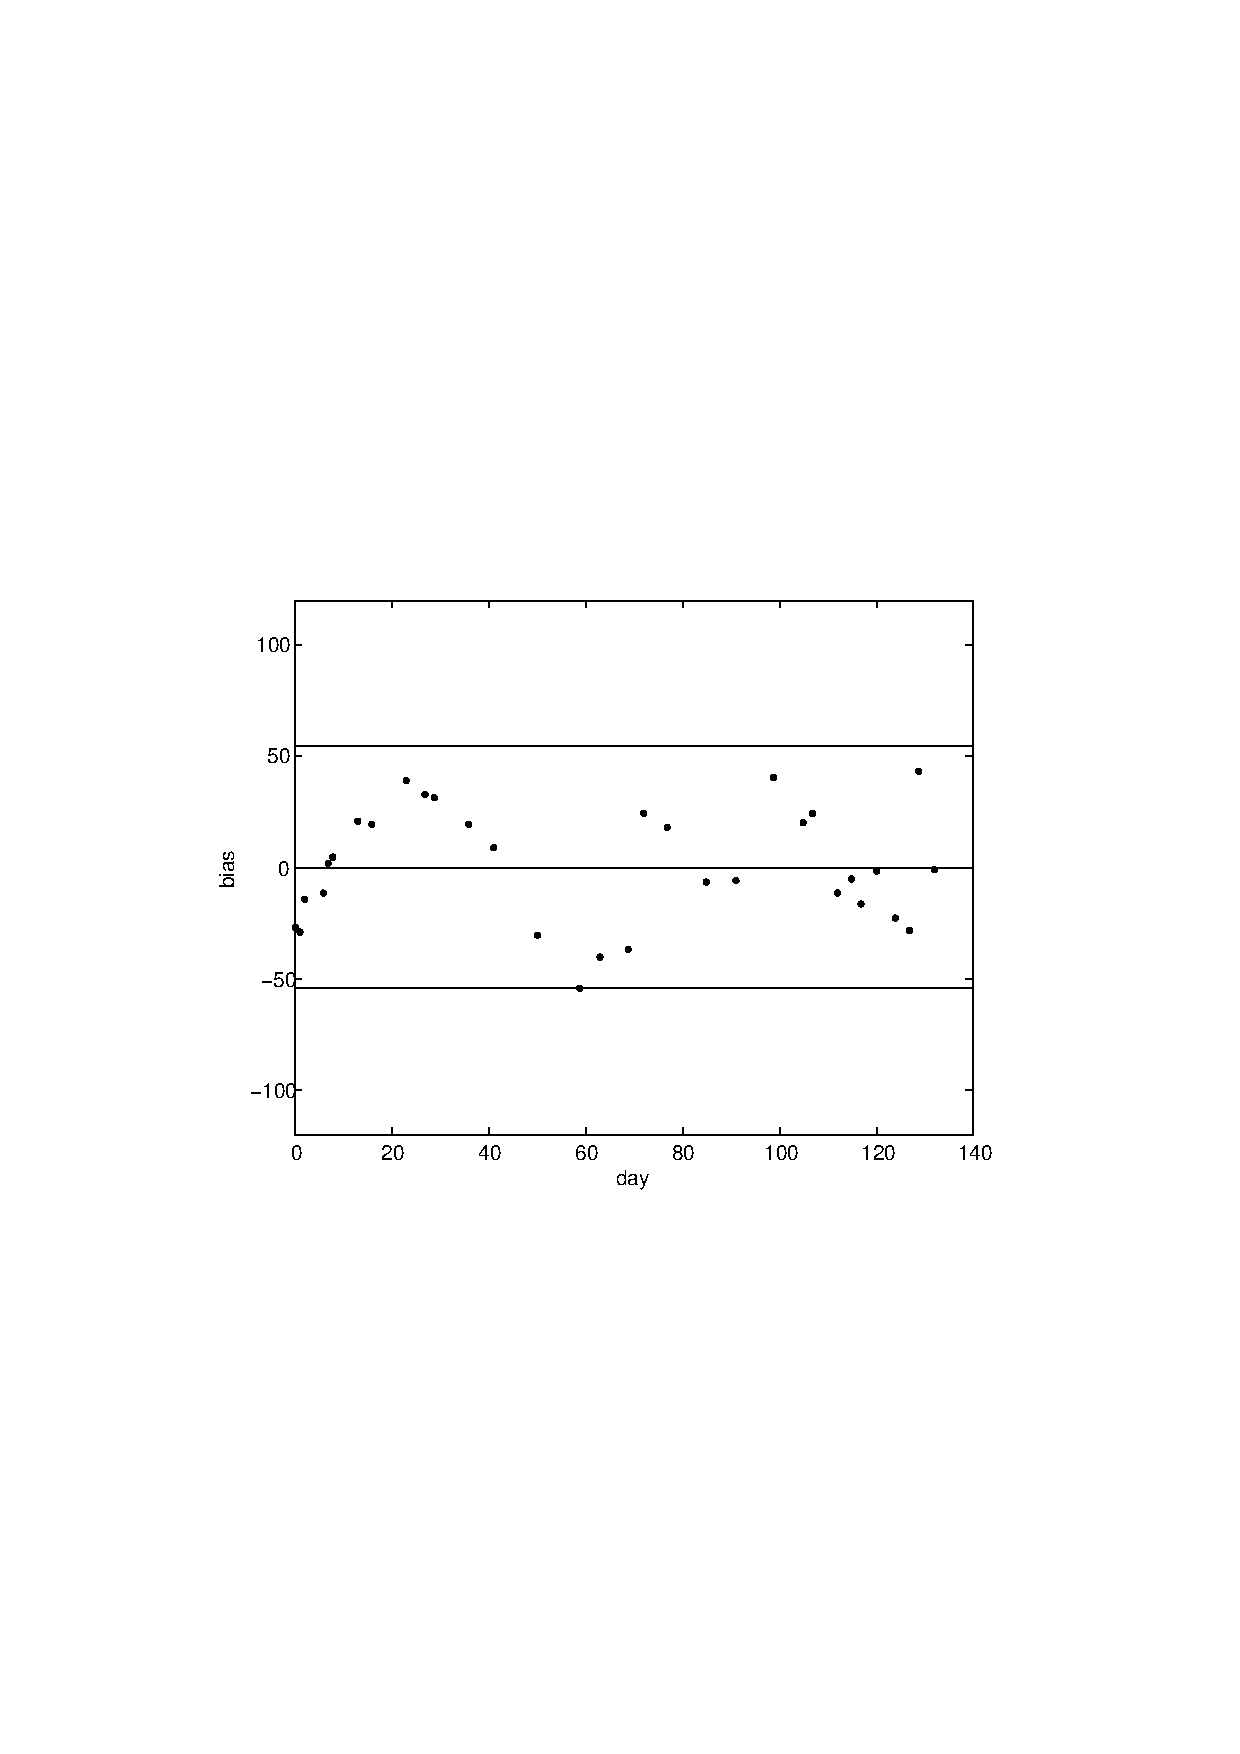
\includegraphics[width=4in]{imgs/cases_fit_bias.pdf}
\caption{Bias analyze.}
\label{fig:6}
\end{figure}
As can be seen from Figure~\ref{fig:6}, the error branch points are
concentrated in the interval $[-55,55]$, so fitting fine,
it shows that the function above in line with the increasement
trend of infectious diseases on beginning, the model has good
fidelity.(MATLAB code for this part is in appendix 5)
